% Copyright (c) 2014, by Yifan Peng <yfpeng@udel.edu>
% All rights reserved.
% 
% Redistribution and use in source and binary forms, with or without
% modification, are permitted provided that the following conditions are met:
% 1. Redistributions of source code must retain the above copyright
%    notice, this list of conditions and the following disclaimer.
% 2. Redistributions in binary form must reproduce the above copyright
%    notice, this list of conditions and the following disclaimer in the
%    documentation and/or other materials provided with the distribution.
% 3. All advertising materials mentioning features or use of this software
%    must display the following acknowledgement:
%    This product includes software developed by the <organization>.
% 4. Neither the name of the <organization> nor the
%    names of its contributors may be used to endorse or promote products
%    derived from this software without specific prior written permission.
% 
% THIS SOFTWARE IS PROVIDED BY <COPYRIGHT HOLDER> ''AS IS'' AND ANY
% EXPRESS OR IMPLIED WARRANTIES, INCLUDING, BUT NOT LIMITED TO, THE IMPLIED
% WARRANTIES OF MERCHANTABILITY AND FITNESS FOR A PARTICULAR PURPOSE ARE
% DISCLAIMED. IN NO EVENT SHALL <COPYRIGHT HOLDER> BE LIABLE FOR ANY
% DIRECT, INDIRECT, INCIDENTAL, SPECIAL, EXEMPLARY, OR CONSEQUENTIAL DAMAGES
% (INCLUDING, BUT NOT LIMITED TO, PROCUREMENT OF SUBSTITUTE GOODS OR SERVICES;
% LOSS OF USE, DATA, OR PROFITS; OR BUSINESS INTERRUPTION) HOWEVER CAUSED AND
% ON ANY THEORY OF LIABILITY, WHETHER IN CONTRACT, STRICT LIABILITY, OR TORT
% (INCLUDING NEGLIGENCE OR OTHERWISE) ARISING IN ANY WAY OUT OF THE USE OF THIS
% SOFTWARE, EVEN IF ADVISED OF THE POSSIBILITY OF SUCH DAMAGE.
\PassOptionsToPackage{rgb}{xcolor}
\documentclass{beamer}

\mode<presentation>
\usetheme{Udel}

\usepackage{alltt}
\usepackage{amssymb}
\usepackage{amsmath}
%\usepackage{beamerprosper}
\usepackage[english]{babel}
\usepackage{booktabs}
\usepackage{calc}
\usepackage{colortbl}
\usepackage{helvet}
\usepackage{mathptmx}
\usepackage{multirow}
\usepackage{pgf}
\usepackage{smartdiagram}
\usepackage{tabularx}
\usepackage{tikz}
\usepackage{ulem}
\usepackage{xmpmulti}

\DeclareGraphicsRule{*}{mps}{*}{}
\DeclareMathOperator*{\argmax}{\arg\max}

\graphicspath{{images/}}
%\setbeamerfont{title}{
%	size=\Large,
%	series=\bfseries,
%	shape=\scshape,
%	family=\rmfamily
%}

\usetikzlibrary{%
  arrows,%
  automata,%
  calc,%
  trees,%
  positioning,%
  chains,%
  shapes,%
  shapes.arrows,%
  shapes.geometric,%
  shapes.misc,% wg. rounded rectangle
  shapes.symbols,%
  decorations.pathreplacing,%
  decorations.pathmorphing,% /pgf/decoration/random steps | erste Graphik
  matrix,%
  scopes,%
  shadows%
 }

%\includeonlyframes{cur}


\title{Beamer Theme with \\University of Delaware Logo (v4)}
\author[Yifan Peng]{Yifan Peng}
\institute[Computer \& Information Sciences]{Computer \& Information
Sciences}
\date[today]{\today}

\pgfdeclarelayer{background}
\pgfdeclarelayer{foreground}
\pgfsetlayers{background,main,foreground}

\begin{document}

\begin{frame}[plain]
    \titlepage
\end{frame}

\begin{frame}
  \frametitle{Outline} 
  \tableofcontents[hideallsubsections]
\end{frame}

\section{UD Colors}

\begin{frame}
	\frametitle{UD Colors}
	\begin{exampleblock}{University Colors}
	\begin{itemize}
	  \item Udel blue: \textcolor{udelblue}{RGB: 0, 83, 159}
	  \item Udel dark blue: \textcolor{udeldarkblue}{RGB: 0, 38, 99}
	  \item Udel yellow: \textcolor{udelyellow}{RGB: 255, 210, 0}
	\end{itemize}
	\end{exampleblock}
\end{frame}

\section{UD Primary Logo}

\begin{frame}
	\frametitle{UD Primary Logo}
	\begin{figure}
		
\includegraphics[width=.5\textwidth]{UDPrimaryLogo2945.pdf}
	\end{figure}
\end{frame}

\section{Diagram}

\begin{frame}[fragile] 
  \frametitle{Graphitemize}
  \begin{figure}
    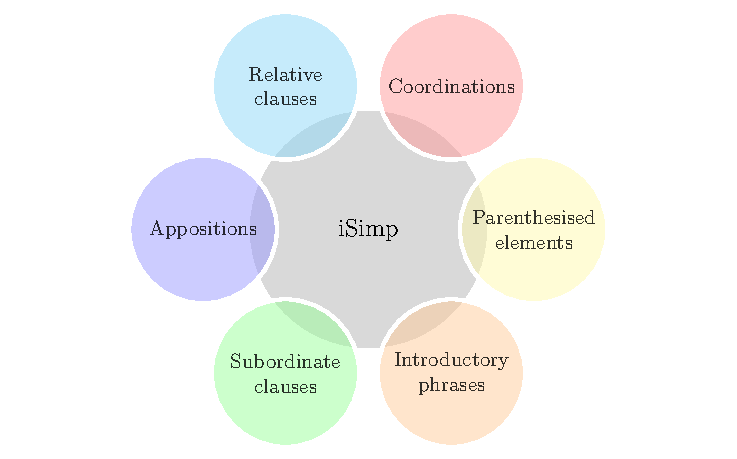
\includegraphics[height=6.8cm,page=1]{bubble.pdf}
  \end{figure}
\end{frame}

\begin{frame}
  \frametitle{Graphitemize}
  \begin{figure}
    \includegraphics[height=6.8cm,page=2]{bubble.pdf}
  \end{figure}
\end{frame}

\begin{frame}[fragile] 
  \frametitle{Linear Flow}
  \begin{figure}
    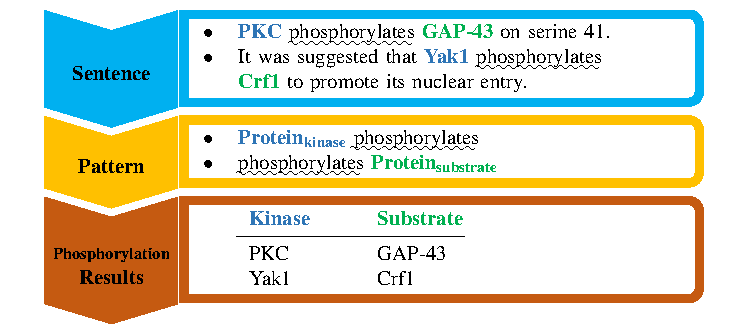
\includegraphics[width=\textwidth,page=1]{linear.pdf}
  \end{figure}
\end{frame}

\begin{frame}
  \frametitle{Linear Flow}
  \begin{figure}
    \includegraphics[width=\textwidth,page=2]{linear.pdf}
  \end{figure}
\end{frame}

\begin{frame}[label=bar,fragile]
	\frametitle{Horizontal Bar Chart}
	\begin{figure}
	  \vspace*{-2em}
	  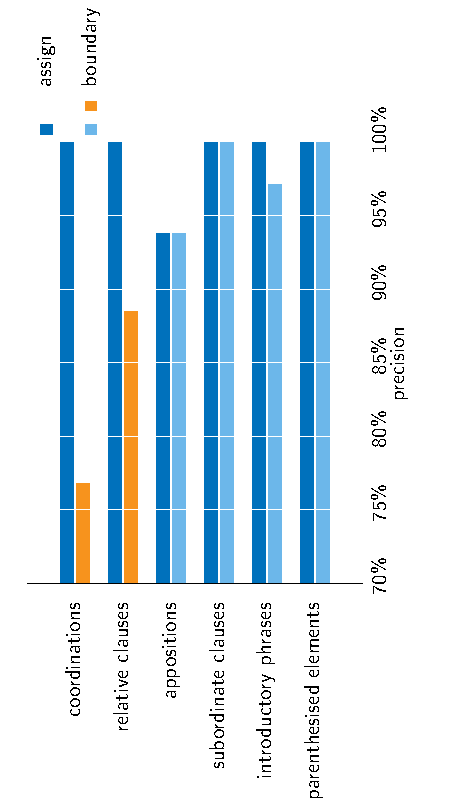
\includegraphics[height=\textwidth,angle=-90]{fvaluemodify.pdf}
	\end{figure}
\end{frame}

\begin{frame}[label=bar2,fragile]
  \frametitle{Horizontal Bar Chart}
  \begin{figure}
    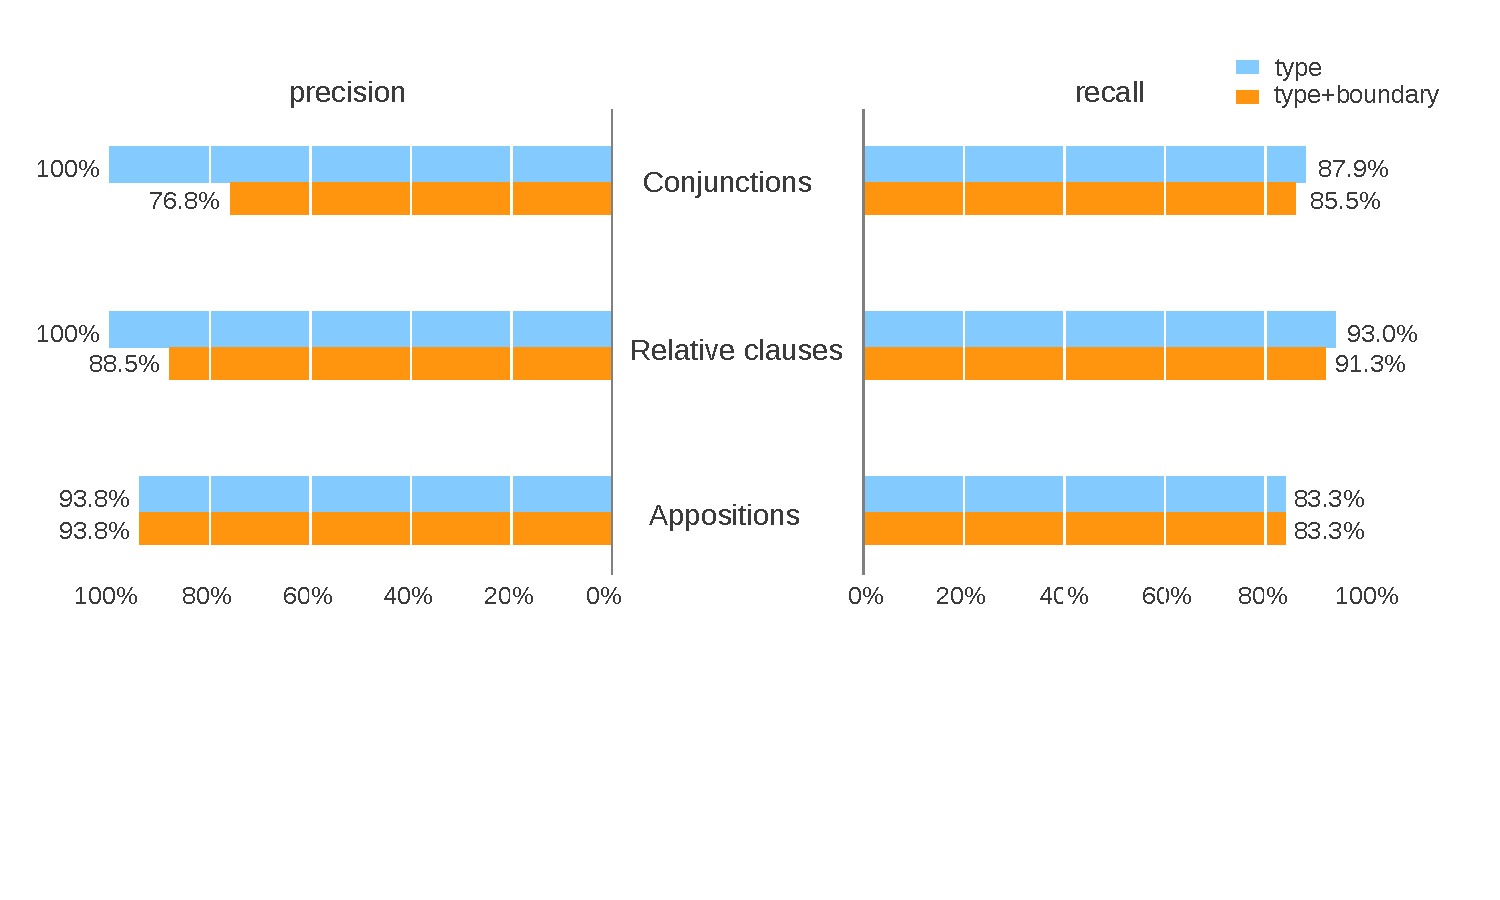
\includegraphics[width=\textwidth]{precision7.pdf}
  \end{figure}
\end{frame}

\begin{frame}[label=color,fragile]
  \frametitle{Color in tables}
  \begin{table}
  \begin{tabular}{l|l}
    \hline
    \rowcolor{udelblue}\color{white}xxxxxxxxxxxxxxxxxx 
      & \color{white}xxxxxxxxxxxxxxxxxxx \\
    \hline
    yyyyyyyyyyyyyy & yyyyyyyyyyy \\
    zzzzzzzzz & zzzzzzzzzz \\
    zzzzzzzzz & zzzzzzzzzz \\
    \hline
  \end{tabular}
  \end{table}
\end{frame}

\begin{frame}[label=colorwheel,fragile]
  \frametitle{Colorwheel}
  \begin{figure}
    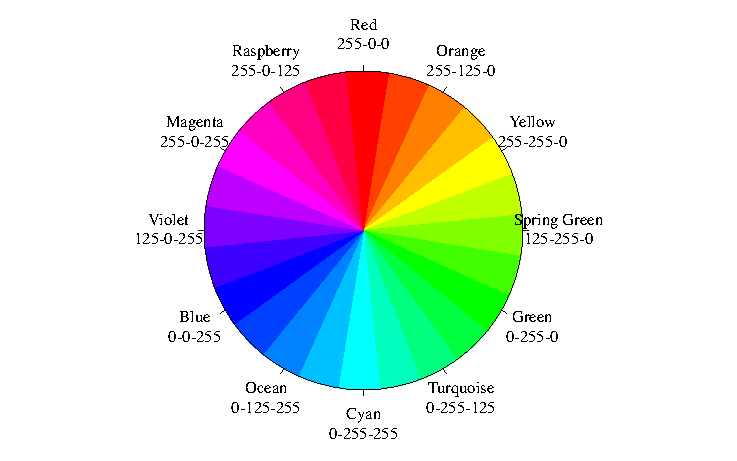
\includegraphics[height=6.8cm]{colorwheel.pdf}
  \end{figure} 
\end{frame}

\begin{frame}
	\frametitle{\;}
  \begin{center}
    \huge Q \& A \vspace{1em}
  \end{center}
\end{frame}

\end{document}
